\documentclass[12pt]{article}
\usepackage{pgfplots, url, tikz, graphicx}
\usepackage{enumitem} % To customize enumerate
\usepackage{amssymb}
\usepackage{caption}
\usepackage{subcaption}
\usepackage{amsmath}
\usepackage{float}
\usetikzlibrary{arrows.meta, positioning}
\pgfplotsset{compat=1.18}

\title{Math HW Week 6}
\author{Duc Nguyen}
\date{\today}

\begin{document}
\maketitle
\section*{Section 3.3}
\subsection*{\#1}
\begin{align*}
    \begin{cases}
    X' = -0.5X \\
    Y' = -Y
    \end{cases}
\end{align*}
\begin{align*}
    \begin{cases}
    0 = -0.5X \\
    0 = -Y
    \end{cases}
\end{align*}
\begin{align*}
    \begin{cases}
    X = 0 \\
    Y = 0
    \end{cases}
\end{align*}
$=> (x,y) = (0,0)$
\subsection*{\#2}
The change vector would just be the vector itself, $(3,-4)$. I don't know which part of the vector should I start, at the origin or at the point $(3,-4)$.

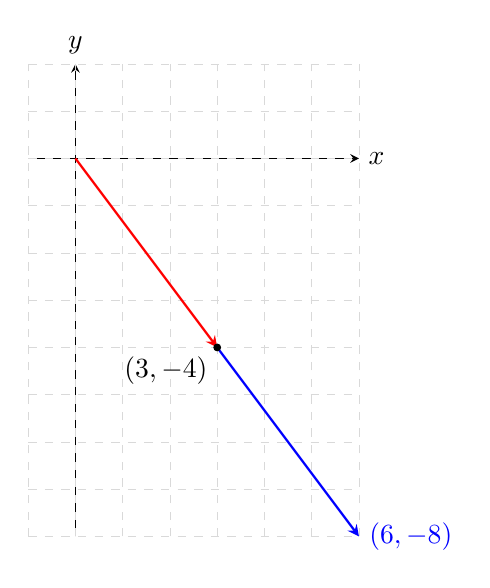
\begin{tikzpicture}[scale=0.6,>=stealth]

    % Axes
    \draw[->] (-1,0) -- (6,0) node[right] {$x$};
    \draw[->] (0,-8) -- (0,2) node[above] {$y$};
    
    % Grid (optional)
    \draw[help lines, color=gray!30, dashed] (-1,-8) grid (6,2);
    
    % Vector at (3, -4)
    \draw[->, thick, red] (0,0) -- (3,-4);

    % Vector from (3, -4)
    \draw[->, thick, blue] (3,-4) -- (6,-8) node[right] {$(6, -8)$};
    
    % Label the point (3, -4)
    \filldraw[black] (3,-4) circle (2pt) node[below left] {$(3, -4)$};
    
\end{tikzpicture}
\subsection*{\#3}
% --- System 1 ---
\begin{center}
    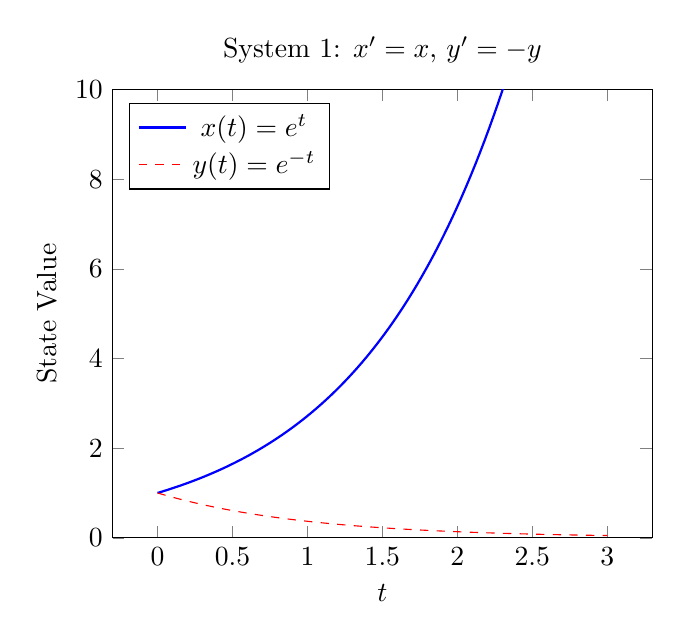
\begin{tikzpicture}
    \begin{axis}[
        title={System 1: $x' = x$, $y' = -y$},
        xlabel={$t$},
        ylabel={State Value},
        legend pos=north west,
        domain=0:3,
        samples=100,
        ymin=0, ymax=10
    ]
    \addplot[blue, thick] {exp(x)};
    \addlegendentry{$x(t) = e^t$}
    
    \addplot[red, dashed] {exp(-x)};
    \addlegendentry{$y(t) = e^{-t}$}
    \end{axis}
    \end{tikzpicture}
\end{center}
    
    \vspace{1cm} % optional spacing
    
    % --- System 2 ---
\begin{center}
    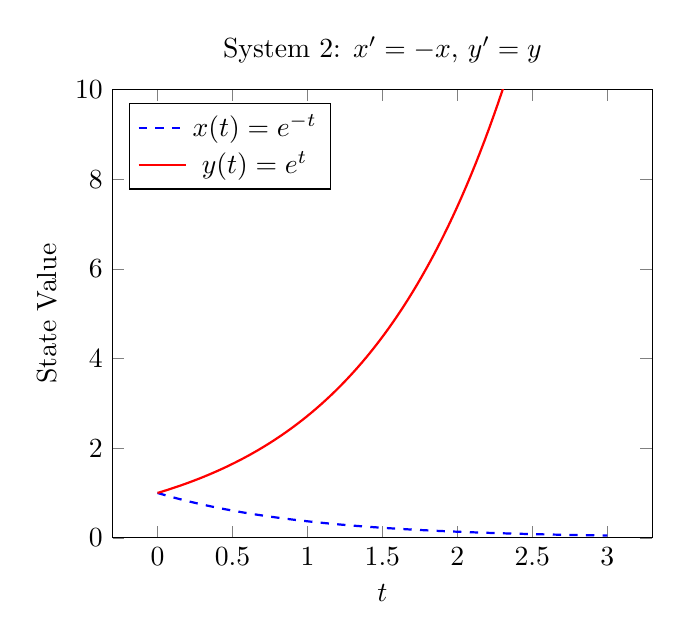
\begin{tikzpicture}
    \begin{axis}[
        title={System 2: $x' = -x$, $y' = y$},
        xlabel={$t$},
        ylabel={State Value},
        legend pos=north west,
        domain=0:3,
        samples=100,
        ymin=0, ymax=10
    ]
    \addplot[blue, thick, dashed] {exp(-x)};
    \addlegendentry{$x(t) = e^{-t}$}
    
    \addplot[red, thick] {exp(x)};
    \addlegendentry{$y(t) = e^t$}
    \end{axis}
    \end{tikzpicture}
\end{center}
\section*{Further Excercises 3.3}
\subsection*{\#1}
\begin{enumerate}[label=\alph*.]
    \item \begin{align*}
        \begin{cases}
        R' = J - 0.1R \\
        J' = -R
        \end{cases}
    \end{align*}
    \begin{align*}
        \begin{cases}
        0 = J - 0.1R => 0.1R = J \\
        0 = -R
        \end{cases}
    \end{align*}
    \begin{align*}
        \begin{cases}
        R = J / 0.1 => 0 = J / 0.1 => J = 0 \\
        R = 0
        \end{cases}
    \end{align*}
    $=> (R,J) = (0,0)$
    \item We'll use:
    \begin{center}
    $(1,1), (1,-1), (-1,1), (-1,-1), (2,2), (2,-2), (-2, 2), (-2,-2)$ 
    \end{center}
    as the initial points.
    
    For the following system: 
    \begin{align*}
        \begin{cases}
        R' = J - 0.1R \\
        J' = -R
        \end{cases}
    \end{align*}

    We'll have, for (1,1):
    \begin{align*}
        \begin{cases}
        R' = 1 - 0.1(1) => R' = 0.9 \\
        J' = -1
        \end{cases}
    \end{align*}
    We'll have, for (1,-1):
    \begin{align*}
        \begin{cases}
        R' = -1 - 0.1(1) => R' = -1.1 \\
        J' = -1
        \end{cases}
    \end{align*}
    We'll have, for (-1,1):
    \begin{align*}
        \begin{cases}
        R' = 1 - 0.1(-1) => R' = 1.1 \\
        J' = 1
        \end{cases}
    \end{align*}
    We'll have, for (-1,-1):
    \begin{align*}
        \begin{cases}
        R' = -1 - 0.1(-1) => R' = -0.9 \\
        J' = 1
        \end{cases}
    \end{align*}
    We'll have, for (2,2):
    \begin{align*}
        \begin{cases}
        R' = 2 - 0.1(2) => R' = 1.8 \\
        J' = -2
        \end{cases}
    \end{align*}
    We'll have, for (2,-2):
    \begin{align*}
        \begin{cases}
        R' = -2 - 0.1(2) => R' = -2.2 \\
        J' = -2
        \end{cases}
    \end{align*}
    We'll have, for (-2,2):
    \begin{align*}
        \begin{cases}
        R' = 2 - 0.1(-2) => R' = 2.2 \\
        J' = 2
        \end{cases}
    \end{align*}
    We'll have, for (-2,-2):
    \begin{align*}
        \begin{cases}
        R' = -2 - 0.1(-2) => R' = -1.8 \\
        J' = -2
        \end{cases}
    \end{align*}

    The sketch of the vector field is represented in d.
    \item They seem to be circulating around the origin
    \item \begin{figure}[!ht]
        \centering
        \includegraphics[width=0.4\textwidth]{vectorField.png} % or .pdf    \end{figure}
    \end{figure}
    \item They have a spiral shape around it
    \begin{figure}[!ht]
        \centering
        \includegraphics[width=0.4\textwidth]{vectorField2.png} % or .pdf
    \end{figure}
\end{enumerate}
\subsection*{\#2}
\begin{enumerate}[label=\alph*.]
    \item \begin{align*}
        \begin{cases}
        R' = J \\
        J' = -R + 0.1J
        \end{cases}
    \end{align*}
    \begin{align*}
        \begin{cases}
        0 = J \\
        0 = -R + 0.1J => R = 0.1J
        \end{cases}
    \end{align*}
    \begin{align*}
        \begin{cases}
        R = 0 \\
        R = 0.1(0) => R = 0
        \end{cases}
    \end{align*}
    $=> (R,J) = (0,0)$
    \item We'll use:
    \begin{center}
    $(1,1), (1,-1), (-1,1), (-1,-1), (2,2), (2,-2), (-2, 2), (-2,-2)$ 
    \end{center}
    as the initial points.
    
    For the following system: 
    \begin{align*}
        \begin{cases}
        R' = J \\
        J' = -R + 0.1J
        \end{cases}
    \end{align*}

    We'll have, for (1,1):
    \begin{align*}
        \begin{cases}
        R' = 1 \\
        J' = -1 + 0.1(1) => J' = -0.9
        \end{cases}
    \end{align*}
    We'll have, for (1,-1):
    \begin{align*}
        \begin{cases}
        R' = -1 \\
        J' = -1 - 0.1(1) => J' = -1.1
        \end{cases}
    \end{align*}
    We'll have, for (-1,1):
    \begin{align*}
        \begin{cases}
        R' = 1 \\
        J' = 1 + 0.1(1) => J' = 1.1
        \end{cases}
    \end{align*}
    We'll have, for (-1,-1):
    \begin{align*}
        \begin{cases}
        R' = -1 \\
        J' = -1 + 0.1(-1) => J' = -1.1
        \end{cases}
    \end{align*}
    We'll have, for (2,2):
    \begin{align*}
        \begin{cases}
        R' = 2 \\
        J' = -2 + 0.1(2) => J' = -1.8
        \end{cases}
    \end{align*}
    We'll have, for (2,-2):
    \begin{align*}
        \begin{cases}
        R' = -2 \\
        J' = -2 + 0.1(-2) => J' = -2.2 
        \end{cases}
    \end{align*}
    We'll have, for (-2,2):
    \begin{align*}
        \begin{cases}
        R' = 2 \\
        J' = 2 + 0.1(2) => J' = 2.2
        \end{cases}
    \end{align*}
    We'll have, for (-2,-2):
    \begin{align*}
        \begin{cases}
        R' = -2 \\
        J' = 2 + 0.1(-2) => J' = 1.8
        \end{cases}
    \end{align*}

    The sketch of the vector field is represented in d.
    \item They seem to be circulating around the origin again, but this time, they are not spiraling to the stable point. They spiraled to the unstable point instead.
    \item \begin{figure}[H]
        \centering
        \includegraphics[width=0.4\textwidth]{vectorField3.png} % or .pdf
    \end{figure}
    \item They have a spiral shape around it like the previous one, but this time, they are not spiraling to the stable point. They spiraled to the unstable point instead as confirmed.
    \begin{figure}[H]
        \centering
        \includegraphics[width=0.4\textwidth]{vectorField4.png} % or .pdf
    \end{figure}
\end{enumerate}
\subsection*{\#3}
\begin{enumerate}[label=\alph*.]
    \item \begin{table}[h]
        \centering
        \begin{tabular}{|c|c|c|}
          \hline
          Value & Behavior \\
          \hline
          $a < -1$ & Approaching equilibrium \\
          $a = -1$   & Approaching equilibrium \\
          $-1 < a < 0$   & Approaching equilibrium \\
            $a = 0$   & Approaching on x-origin \\
            $a > 0$   & Move away \\
          \hline
        \end{tabular}
      \end{table}
      The stability depends on the sign, not the value of $a$. (negativity is more stable than positivity)
      
      If you swap a with d, the stability is the same but with a mirrored effect.
      \item If a and d are both negative, it will show a negative slope, therefore it's more stable. If a and d are both positive, it will show a positive slope, therefore it's more unstable. If they have opposite signs, they will somehow converge to the origin, which also the equilibrium point, depends on the stability of the axis. I guess the stability would be neutral, at that point.
      \begin{figure}[H]
        \centering
        \includegraphics[width=0.4\textwidth]{vector5.png} % or .pdf
        \caption{Vector field with a = 0.5, d = 0.5}
        \label{fig:vector5}
        \end{figure}
        \begin{figure}[H]
            \centering
            \includegraphics[width=0.4\textwidth]{vector6.png} % or .pdf
            \caption{Vector field with a = -0.5, d = -0.5}
        \label{fig:vector6}
        \end{figure}
        \begin{figure}[H]
            \centering
            \includegraphics[width=0.4\textwidth]{vector7.png} % or .pdf
            \caption{Vector field with a = -0.5, d = 0.5}
        \label{fig:vector7}
        \end{figure}
        \begin{figure}[H]
            \centering
            \includegraphics[width=0.4\textwidth]{vector8.png} % or .pdf
            \caption{Vector field with a = 0.5, d = -0.5}
        \label{fig:vector8}
        \end{figure}
        \item By mani pulating b and c, when a and d is positive, b and c will transition from unstable to stable if you cross from negative to positive. When a and d is negative, b and c will transition from stable to unstable if you cross from negative to positive. If a and d have different signs, b and c at 0 will create flow that's unstable to the equilibrium point, but when transition from negative to positive, the flow gets more stable to their respective side, if they're negativem then the flow will flow to the more stable, if they're positive, then the flow will flow to the more unstable side.
\end{enumerate}

\end{document}